\documentclass[a4]{book}
%\documentclass[landscape,twocolumn,a4]{article}

% Package imports
\usepackage[dvipdfm,twocolumn]{geometry} % for 2-column layout
\usepackage{siunitx} % for \SI and \num macro
\usepackage[table]{xcolor} % for \DefineNamedColor
\usepackage{xspace} % for fixing spacing after abbreviations
\usepackage{hyperref} % for all the URLs
\usepackage{float} % for float options like "H"
\usepackage{pdflscape} % set PDF to landscape mode
\usepackage{etoolbox} % for \newbool and \ifbool
\usepackage{environ} % needed, but ... how?
\usepackage{tabu} % for our tables
\usepackage{tikz} % for out images
\usepackage{eso-pic} % for AddToShipoutPicture

% We can remove these once the title box disappears
\usepackage{pifont} % for title-box warning font
\usepackage{mdframed} % for title-box warning frame

\usetikzlibrary{calc}



% Make better use of the page
\geometry{% A4
	papersize={210mm,297mm},
	textwidth=162mm,
	textheight=260mm,
	inner=29mm,
	top=15mm,
	columnsep=15mm,
	footskip=2mm,
}


% Prevent orphans and widows
\clubpenalty = 10000
\widowpenalty = 10000
\displaywidowpenalty = 10000
\finalhyphendemerits = 10000
\brokenpenalty = 7500


% Misc paragraph settings.
\pretolerance 2500
\tolerance 500
\hyphenpenalty 250
\exhyphenpenalty 100
\doublehyphendemerits 7500
\finalhyphendemerits 7500
\lefthyphenmin 3
\righthyphenmin 3
\looseness 1


\setlength\parindent{0pt}


% Add background picture
\AddToShipoutPicture{
\ifthenelse{\isodd{\value{page}}}%
{
    % If we are on an odd / front page
    \put(0,0){\parbox[b][\paperheight]{\paperwidth}{\vfill\centering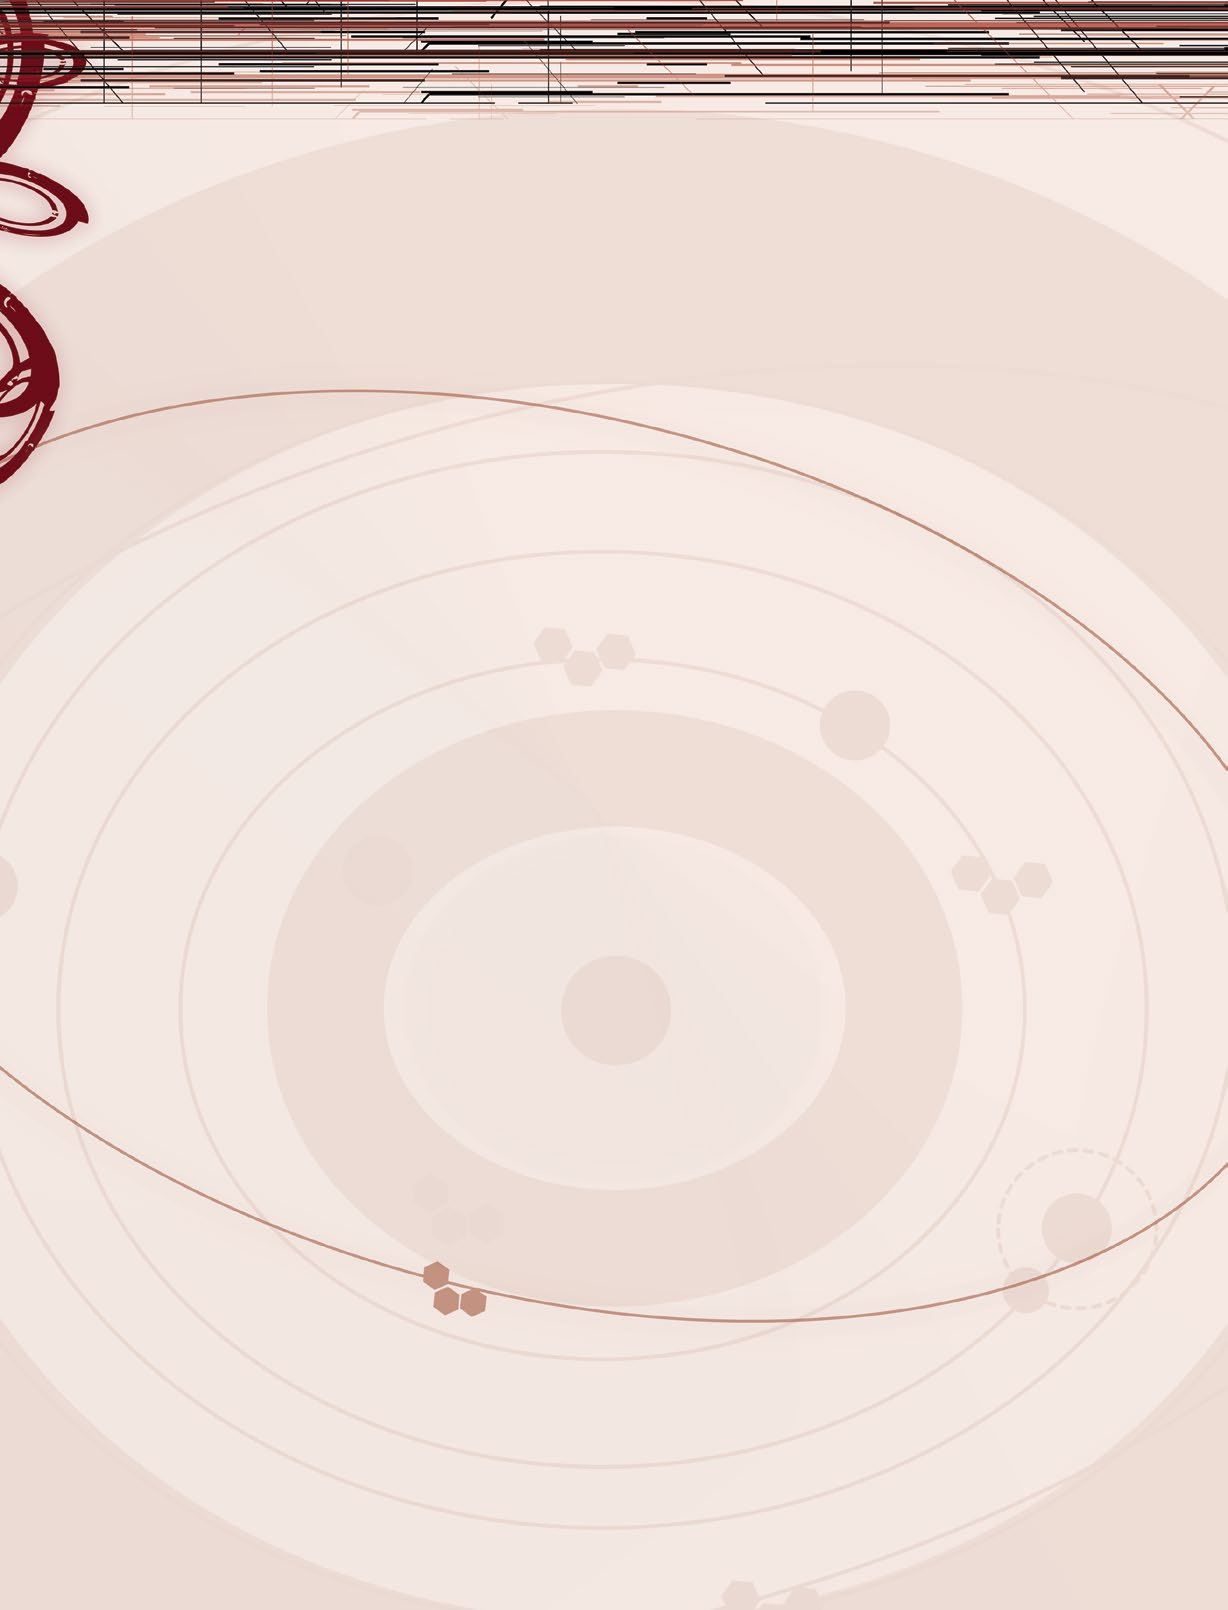
\includegraphics{gfx/backgroundL.jpg}\vfill}}

    \begin{tikzpicture}[remember picture, overlay]
		% If we have single-column
        % \draw[fill=white,color=white,opacity=0.9] (2.5,0) rectangle (19.5, 290);;

		% If we have two-column
		\draw[fill=white,color=white,opacity=0.9] (2.5,0) rectangle (10.7, 290);;
        \draw[fill=white,color=white,opacity=0.9] (11.5,0) rectangle (19.5, 290);;
    \end{tikzpicture}%

}{
    % If we are on an even page
    \put(0,0){\parbox[b][\paperheight]{\paperwidth}{\vfill\centering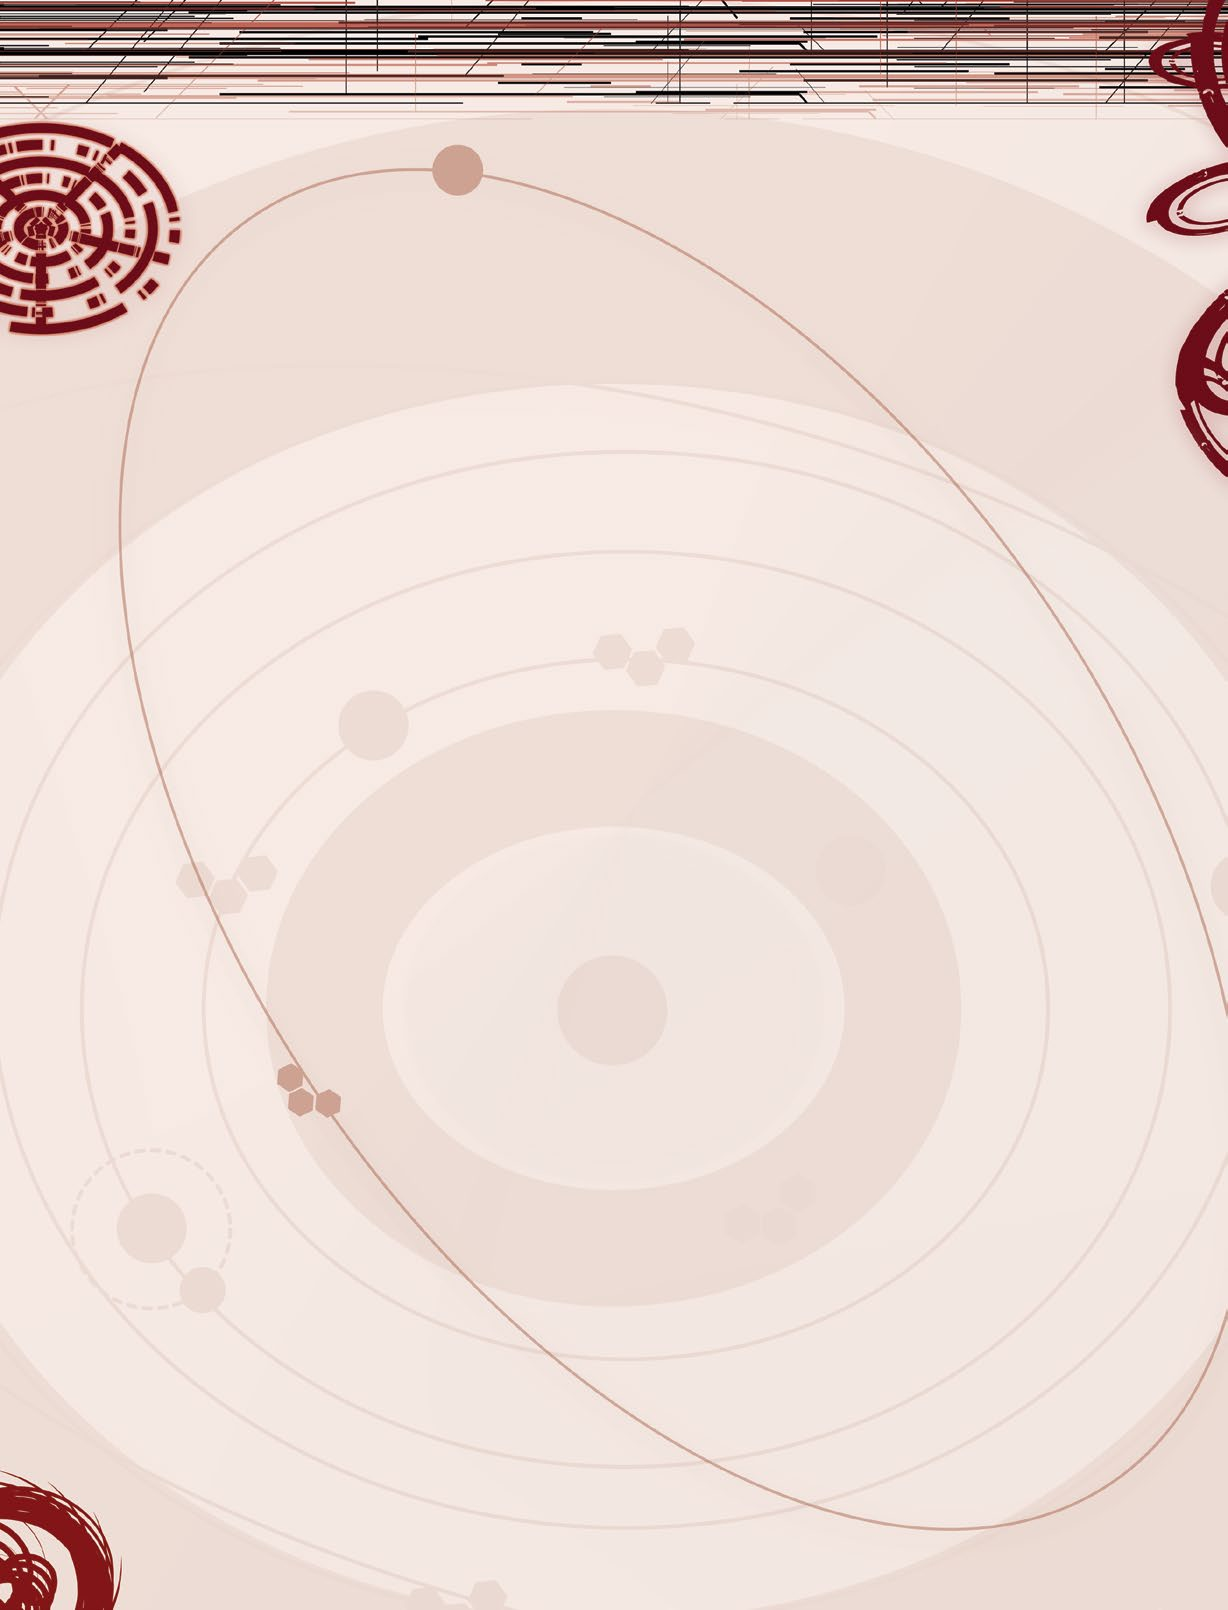
\includegraphics[width=\paperwidth,height=\paperheight]{gfx/backgroundR.jpg}\vfill}}

    \begin{tikzpicture}[remember picture, overlay]
		% If we have single-column
        % \draw[fill=white,color=white,opacity=0.9] (1.6,0) rectangle (18.2, 290);;

		% If we have two-column
		\draw[fill=white,color=white,opacity=0.9] (1.6,0) rectangle (9.6, 290);;
        \draw[fill=white,color=white,opacity=0.9] (10.6,0) rectangle (18.2, 290);;

    \end{tikzpicture}%
}%
}

% hiermit erzwingen wir RGB-rendering und damit treffsicherere Farben, wenn transparenzen im Spiel sind
\AddToShipoutPicture{%
\makeatletter%
\special{pdf: put @thispage <</Group << /S /Transparency /I true /CS /DeviceRGB>> >>}%
\makeatother%
}


\AtBeginShipout{%
}



% COLORS
\DefineNamedColor{named}{eclipsered}{rgb}{0.686,0.066,0.082}
\definecolor{tablecolor}{named}{eclipsered}


% CUSTOM COMMANDS AND ABBREVIATIONS
\newcommand{\todo}[1]{{\color{red} TODO: #1} \typeout{TODO TODO TODO #1}}
\newcommand\nobrkhyph{\mbox{-}}

\newcommand{\dice}[1]{{#1}}
\newcommand{\skill}[2][]{{\ifthenelse{\equal{#1}{}}{#2}{#2\,(\num[retain-explicit-plus]{#1})}}}
\newcommand{\modifier}[1]{{\num[retain-explicit-plus]{#1}}}
\newcommand{\dv}[1]{{DV\,#1}}

\def\eclipsephase{Eclipse Phase\xspace}
\def\ep{EP\xspace}




% For abbreviations such as i.e., e.g., …
% Also, omit final dot from each def.
\ExplSyntaxOn
\newcommand\latinabbrev[1]{
  \peek_meaning:NTF . {% Same as \@ifnextchar
    #1\@}%
  { \peek_catcode:NTF a {% Check whether next char has same catcode as \'a, i.e., is a letter
      #1.\@ }%
    {#1.\@}}}
\ExplSyntaxOff

\def\eg{\latinabbrev{e.g}}
\def\etal{\latinabbrev{et al}}
\def\etc{\latinabbrev{etc}}
\def\ie{\latinabbrev{i.e}}


% TABLES
\newsavebox{\tablebox}
\preto\tabu{\setcounter{magicrownumbers}{0}}
\newcounter{magicrownumbers}
\newcommand\rownumber{\stepcounter{magicrownumbers}\arabic{magicrownumbers}}

% Base fancy Eclipse Phase box
% https://tex.stackexchange.com/questions/78692/using-an-environ-environment-with-newenvironment
\environbodyname\rndtablebody
\NewEnviron{rndtable}[1]{%

    % Alternating background rows
    %\rowcolors{2}{tablecolor!10}{tablecolor!30}%
    \taburowcolors[2]{tablecolor!10 .. tablecolor!30}%
    % \addtolength{\extrarowheight}{0.3ex}%
    % \addtolength{\extrarowdepth}{0.3ex}%

    % Actual table content
    % WTF DO I NEED '%' at the end of these lines since otherwise it will look ugly?
    \savebox{\tablebox}{%
        \begin{tabu}[htbp]{#1}%
            \rndtablebody%
        \end{tabu}%
    }%

    % Fancy frame
    \begin{tikzpicture}
        \begin{scope}
          \clip[rounded corners=1ex] (0,-\dp\tablebox) -- (\wd\tablebox,-\dp\tablebox) -- (\wd\tablebox,\ht\tablebox) -- (0,\ht\tablebox) -- cycle;
          \node at (0,-\dp\tablebox) [anchor=south west,inner sep=0pt]{\usebox{\tablebox}};
        \end{scope}
        \draw[rounded corners=1ex] (0,-\dp\tablebox) -- (\wd\tablebox,-\dp\tablebox) -- (\wd\tablebox,\ht\tablebox) -- (0,\ht\tablebox) -- cycle;
    \end{tikzpicture}

}


% Table with one column
\environbodyname\tableonebody
\NewEnviron{tableone}[1]{
    \begin{rndtable}{ X }
        \multicolumn{1}{c}{
            \cellcolor{tablecolor}\color{white} \Huge{#1}
    } \\
    \hline
    \tableonebody
    \end{rndtable}
}


% Table with two columns, one of which is row number
\environbodyname\tabletworndbody
\NewEnviron{tabletwornd}[1]{
    \begin{rndtable}{ l | X }
        \multicolumn{2}{c}{
            \cellcolor{tablecolor}\color{white} \Huge{#1}
    } \\
    \hline
    \tabletworndbody
    \end{rndtable}
}


% Table with two columns
\environbodyname\tabletwobody
\NewEnviron{tabletwo}[1]{
    %\begin{rndtable}{p{0.25\columnwidth} | p{0.7\columnwidth} }
    \begin{rndtable}{ l | X }
        \multicolumn{2}{c}{
            \cellcolor{tablecolor}\color{white} #1
    } \\
    \hline
    \tabletwobody
    \end{rndtable}
}



\begin{document}
\title{The Lost Transmission}


\section{Stations}

Blah bluss

\input{ch.gmtips}

%%%
%%%
%%% WORKING AREA1
%%%
%%%

\begin{multicols}{2}

\section*{General GM Tips}
\subsection*{Fantasy Tropes in Eclipse Phase}


\eclipsephase can be daunting to GM at first, in particular when coming from a fantasy background.
%
Many \textit{tropes} require different game play elements to produce similar results.
%
Here are some tips to convert some of them to the \eclipsephase universe.

\medskip

For example:
``The heroes travel along a lonely road through the forest.
They find the remains of an ambush site.
A wounded survivor tells them a princess was captured by an evil mage and is kept in an old tower.
Being too far away from the next town to call for help, he urges the players to rescue her.
The players sneak into his evil tower, fight the mage, and eventually rescue the princess.
They are being handsomely rewarded.``

In the \eclipsephase:

\end{multicols}

\begin{tabletwo}{Locations}
    Bandits & Gang (A, B). Pirates (X, Y, Z). Conflicting Faction (Brinkers, X). Spies (Jovian Republic).\\
    Monster Encounters & Automated Security Systems (X). AI (various morphs). Gamma Forks. (Not-quite) Uplifts. Infected (X-Risks). Nano swarms.\\
    Ambush & xxx \\
    Nature \& Forest & Rock Formations. Terraformed Micro Climate. Stations. Hydroponics. Parks. Exoplants. Derelict Station Parts. \\
    Pacing & Generally `one order of magnitide` faster in \ep (weeks become days, days become hours). \textit{Three days in dungeon} becomes \textit{3 hours in old ventilation system}.\\
    Succeeding \& Failing & Related to Pacing. If players have time, they will (should reasonably) succeed. Implication: In many cases \textit{adventure} / challenge only arises if there is less time than needed. \\
    Being Lost & Actually Lost (away from civilization, unknown habitat). Factually Lost (recently reworked structure, unknown / moving target) \\
    Maps & Available except special events (major disaster, very old station part, Earth, Exoplanet). \\
    Being Alone & Totally Alone (interference, radio transmitter outside Mesh range, Exoplanet). Physically Alone (help takes too long to arrive).\\
    Exploring the Dungeon & Derelict Ships. Old Station Parts. Earth. Exoplanet Ruins. Habitats w/o Clearance (\eg, gang territory, private dwellings).\\
    Resting \& Healing & Morph damage only scary w. tight pacing (timeframe hours). Ego damage much more severe (timeframe weeks). Also remember to apply hardening (permanent)! \\
    Death & Regular death in \ep needs additional story consequences (\eg, target escaped, Stack popped by enemy, too late for rendezvous, exoplanet and no spare morphs left)! \\
    Death (Final) & Exurgent Virus (the ultimate threat: use sparingly, loses edge).\\
    Murder Plots & Depends on victim stratum (rich: usually had good backup, middle class: also required popped stack and no backup, very low or Jovian: might be dead for real). \\
    Kidnapping & Becomes Forknapping. Often more scary than murder. \\
    Sneaking & Situation dependent. Alternatively Blend In (passcoes)  \\
    Magic & Infosec (Hacking, AR) . Military Technology. AGIs. Exsurgent Virus. Asyncs. \\
    %Vendors \& Items & . \\
    Gold \& Rewards & Information (multi-use blueprints, single-use expensive). Reputation. Contacts. Restricted Items (weapons, weapon blueprints). Morphs. Apartments. Vehicles. Ships.\\
    %Heroism & Must be agreed out-of-game. Firewall implies certain heroism. \\
    The Princess &  \\
\end{tabletwo}


\begin{multicols}{2}

\section*{Plot Hooks}

\end{multicols}


\begin{tableone}{Locations}
Firwall and the fight of X-Risks.\\
Salvage or retrieval of weapon systems.\\
\textellipsis physical resources.\\
\textellipsis lost databanks.\\
\textellipsis left-behind uploads of friends \& family.\\
\textellipsis important people.\\
\textellipsis tech- nologies developed and lost in the brief singularity takeoff.\\
\textellipsis valued heirlooms of immortal oligarchs.\\
\textellipsis someone who needs to be saved, or is beyond saving.\\
Exploration of Kuiper Belt.\\
\textellipsis of Pandora Gates.\\
\textellipsis of isolationist posthuman factions.\\
\textellipsis of secretive criminal cartels.\\
\textellipsis of pirates.\\
\textellipsis of aliens.\\
Trade of information.\\
\textellipsis favors.\\
\textellipsis creativity.\\
Crime, such as informorph slave trading.\\
\textellipsis pleasure-pod sex industries.\\
\textellipsis data brokerage \& theft.\\
\textellipsis extraction of tech \& scientists.\\
\textellipsis smuggling of technologies.\\
\textellipsis political \& corporate espionage.\\
\textellipsis assassination.\\
\textellipsis drug \& XP dealing.\\
\textellipsis soul trading.\\
Mercenary work related to faction struggles.\\
\textellipsis contested resources.\\
\textellipsis colonization beyond Pandora gates.\\
\textellipsis raids.\\
\textellipsis commando operations.\\
Socio-political intrigue between factions.\\
\textellipsis hypercorps.\\
\textellipsis governments.\\
\textellipsis habitats.\\
\end{tableone}

\begin{multicols}{2}

\section*{Locations}

Design criteria.

\begin{itemize}
    \item Copious use of \textit{distant mountain.s}
    \item Logically derive from official \eclipsephase lore.
    \item Don't interfere with story hooks, but provide them.
\end{itemize}

\subsection*{Habitat} Planet, Station Type (cylinder, cole), Location (inner, outer, ...)
\subsection*{Economy} Old, Trans, New
\subsection*{Politics} Factions, ...
\subsection*{Governance} Vote, Junta, ...
\subsection*{Security} Weapons avail, just some, ...
\subsection*{Law \& Order} Private, Public, ...
\subsection*{Fabber Access} no, limited, unrestricted


\end{multicols}{2}



\begin{multicols}{2}

\section*{Habitat Building}

Basic idea: GM defines room of type

\subsection*{Transportation \& Access}

Transportation and access systems are usually the first ones players will encounter
traveling to a new habitat.
\end{multicols}{2}


\begin{tableone}{Locations}
Small hangar for storing (6 ground craft, 2 shuttles).\\
Medium hangar for storing (20 ground craft, 6 shuttles).\\
Large hangar for storing (100 ground craft, 20 shuttles).\\
Huge hangar for storing (1000 ground craft, 100 shuttles).\\
Shut down hangar containing no vehicles.\\
Shut down hangar containing a few damaged vehicles.\\
Shut down hangar containing one vehicle in pristine condition.\\
Rail-based transit system connecting different wings of the hab.\\
Capsule based transit system running in three dimensions.\\
Tunnel system for ground vehicles and transport drones.\\
Network of walking escalators connecting the local wing of the hab.\\
High speed transport system for tiny morphs and drones spreading through the hab.\\
Liquid filled transport tubes for aquatic morphs.\\
Tiny maintenance airlock for a \todo{mini morph}.\\
Small maintenance airlock capable of cycling a single person.\\
Airlock for a group of 3 - 6 people.\\
Large airlock for a dozen of people or a single vehicle.\\
Gigantic airlock for two dozen of people and multiple vehicles.\\
Airlock made of nano-tissues allowing characters to permeate slowly.\\
Locked down airlock due to maintenance.\\
Airlock welded shut.\\
Airlock breached and sealed after previous incident.\\
Sealed hull breach. Can be reopened, at risk of uncontrolled decompression.\\
A bodybank / resleeving facility.\\
As above, with attached farcaster port.\\
\end{tableone}



\begin{multicols}{2}


\subsection*{Living \& Recreational}

Living and recreational facilities are where most inhabitants spend most parts of their life.

Room Types

\end{multicols}


\begin{tableone}{Locations}
Tiny space made for \todo{tiny pods}.\\
Cramped one-room apartment.\\
Regular sized one-room apartment.\\
Two-room living space.\\
Three-room living space for a family.\\
Four-room living space for a large family.\\
Detached station part including multiple rooms.\\
Flooded space made for crab pods.\\
Merely a \textit{parking spot} and power connector for a synth morph.\\
Larger \todo{...} for avian morphs.\\
Museum, displaying genuine Earth relics.\\
Museum, displaying genuine specimen from Pandora Gates.\\
A (soccer, tennis, basketball) court.\\
Skydiving.\\
Church.\\
Large, fractal tank of water used recreationally and with rooms for living octopi.\\
Morph racing.\\
\todo{Mech-case} combat.\\
Pleasure pod hotel.\\
VIP lounge.\\
Street food vendor.\\
Restaurant where locals meet with the hab's best pan pizza.\\
Upper-class restaurant with a nice view.\\
Shop selling handmade (clothing, paintings, sculptures).\\
Vehicle vendor near on of the hab's ports.\\
\end{tableone}


\begin{tableone}{Contents}
% Contains
Has latest furniture created by (Venusian, Jovian, ...) designers.\\
Full with actual posters of Venusian Cloud Diving.\\
Pirated stick containing latest, unreleased XP action movies.\\
Has miniature models of two dozen synth morph variants.\\
An old medal indicates a relative was involved in early AGI research.\\
% See
The room has a nice view (into space, over the city, ... ).\\
There are fresh blood splatters on the wall.\\
Nano-swarm is disassembling a plant.\\
% Smell
Faint scent of leaked oil is in the air.\\
Bathroom vent smells like sewage.\\
Smell of recent sex hangs in the air.\\
Scent of spices hints at a meal that was prepared just recently.\\
% Hear
A faint humming of the station's power generator is audible.\\
Neighbors can be heard having an argument.\\
Neighbors can be heard listening to extremely loud music.\\
Neighbors can be heard having a party.\\
% Feel
Walls are coated in a nano-texture that is cold to the touch.\\
A big table made of rough, uneven marble stands in center.\\
% Taste
A metallic taste lingers in the air.\\
A bowl in the fabber contains bitter-tasting cookies.\\
% AR
AR picture frames only show static.\\
The room is full of intrusive AR payday loan ads.\\
The room is physically empty but neatly furnished in AR.\\
The room is devoid of any AR tag.\\
Several AR newsfeeds are pinned to a wall related to char's previous actions.
% Muse
% Events
A neighbor exceeded her quota, she asks to fab item.\\
A small \todo{crab} morph hidden in the corner that mistook you for intruders.\\
Hab security was (accidentally?) alerted to your entry.\\
Players find RFID tag that can unlock a nearby apartment.\\
\end{tableone}


\begin{multicols}{2}

\subsection*{Production \& Research}

Production and research facilities provide a unique backdrop to the world, and
enable players to explore what drives the future world.

Room Types
\end{multicols}

\begin{tableone}{Locations}
Highly secured backup insurance site.\\
Plasma research.\\
Nano research.\\
Weapons research.\\
Propulsion research.\\
Antimatter research.\\
AI research.\\
Xenobiology research.\\
Factor research.\\
Geological.\\
Stellar.\\
Particle accelerator.\\
Quantum.\\
Uplift.\\
The Fall.\\
TITANs.\\
Elemental processor extracting fabber capsules.\\
Material testing facility.\\
Production facility for vehicles.\\
(Mining, drilling) facility.\\
\textellipsis habitat parts.\\
\textellipsis space propulsion systems.\\
\textellipsis terraforming machinery.\\
\textellipsis \todo{fancy material}.\\
\textellipsis advanced computer \& mesh parts.\\
\textellipsis mass production of small arms.\\
\textellipsis ship weapons.\\
Hydroponics farm growing (corn, wheat, rice).\\
\textellipsis spices.\\
\textellipsis legal drugs.\\
Chemical plant producing oxidizers.\\
\textellipsis ultra pure \todo{nanite} base.\\
Power plant operating on solar energy.\\
\textellipsis thermal energy.\\
\textellipsis fusion.\\
\textellipsis fission.\\
\textellipsis antimatter.\\
Automated farm raising (cows, chicken), producing meat.\\
Synthetic morph production facility.\\
Biomorph production facility.\\
\end{tableone}


Sizes

\begin{tableone}{Locations}
One large hall.\\
Several large halls connected (underground, via skyway).\\
A (building, station section), not generally accessible.\\
Consisting of several large (buildings, station arms).\\
Occupying most of the habitat.\\
\end{tableone}



Room Contents

\starttableone
% Contains
% See
% Smell
% Hear
% Feel
% Taste
% AR
% Muse
% Events
\stoptableone


\begin{multicols}{2}

\subsection*{Mesh \& VR}

Unbound by physical constraints, VR worlds provide a place for work and escape.

\end{multicols}{2}

\begin{tableone}{Locations}
A lush park.\\
Office spaces overlooking (Paris, New York, Tokyo).\\
Camp near Great Pyramids in eternal sunset.\\
An exact replica of the encompassing habitat.\\
A \textit{design sweat shop} run by criminals, feeding hype for latest trends.\\
Dante's Inferno.\\
An aerostat over Patagonia.\\
A creative place for \todo{hypercorp}.\\
Recruitment for \todo{hypercorp}.\\
\end{tableone}


\starttableone
% Contains
% See
% Smell
% Hear
% Feel
% Taste
% AR
% Muse
% Events
\stoptableone



\subsection*{Services \& Security}

\begin{tableone}{Locations}
Control center managing section maintenance.\\
Control center managing public security feeds.\\
Control center managing security access.\\
Control center managing energy distribution.\\
Control center managing local traffic.\\
Control center managing regional traffic.\\
Vessel's bridge managing all of the above.\\
Small booth housing a security drone.\\
Security office with 1 - 6 officers.\\
A fully automated \todo{bio tank} facility.\\

Local jail.\\
Trauma hospital.\\
Prison complex.\\
Secured prison node with simulspace storage.\\
Missile storage for one of the ship's / hab's weapon system.\\
Mass driver storage and feeds for ship's / hab's phalanx system.\\
\end{tableone}



\begin{tableone}{Locations}
After resleeving, the character is disoriented and unsure which year it is.\\
After farcasting / resleeving, two weeks are mysteriously missing.\\
As above, and the player's morph was upgraded to a better model.\\
As above, and the player's morph was downgraded to an inferior model.\\
The new morph comes with an addiction.\\
Player learns an old friend / love has recently resleeved here.\\
The morph comes with complimentary facial surgery to make Ego feel more at home.\\
The mirror in the waking chamber has a crack at face height as if from a punch.\\
The player bumps his (head, ellbow, shoulder) the first time he leaves the room.\\
\end{tableone}



\begin{multicols}{2}


\subsection*{Maintenance}

Dark tunnels and a lack of traffic \todo {...}

\end{multicols}{2}

\begin{tableone}{Locations}
Fresh water distribution system.\\
Sewage system.\\
Waste water treatment.\\
Maintenance tunnel network.\\
Hazardous material processing facility.\\
Abandoned parts of previous station.\\
Drone access hatch.\\
Power supply lines and section controls.\\
A Mesh backbone node.\\
Ventilation tunnels (with extreme UV air filtering).\\
(Abandoned, Stand-by, Occupied) emergency shelter.\\
Construction site, preparing for hab extension.\\
\end{tableone}

\begin{tableone}{Locations}
% Contains
% See
% Smell
% Hear
% Feel
% Taste
% AR
% Muse
% Events
A runner for \todo{underground org} passes through.\\
\end{tableone}






\subsection*{Countryside}
% Mars, Luna, Titan, ...

\begin{tableone}{Locations}
Large crater.\\
Habitat is being constructed.
Massive terraforming towers circulate air.\\
Abandoned settlement.\\
Ranger outpost on landmark overlook large parts of the plains.\\
Small, destroyed habitat due to (landslide, impact, explosion).\\
Rail system connecting habitats.\\
Long straight road with little traffic.\\
Small serpentines leading to a tin can down a crater.\\
Two satellite dishes and aimed at different locations in the sky.\\
Operational or abandoned mine.\\
Excarvation site.\\
Small emergency dome (\SI{3}{\m}) errected.\\
(Mars) Cave with microclimate and unusual plant life.\\
\end{tableone}


\begin{tableone}{Locations}
% Contains
Tire tracks disappearing.\\
Burn marks of a recent shuttle landing.\\
% See
Movement can be seen on the horizon.\\
% Smell
% Hear
% Feel
% Taste
% AR
% Muse
% Events
Shuttle passes over the player's heads.\\
Micrometeorite impacts a few meters away, leaving a suspended dust cloud.\\
\end{tableone}



\subsection*{Space}

Random encounters in open space are very unusual given the large distances and high relative speeds.
Most of the sites below are meant to be explicitly targeted, not encountered \textit{along the way}.
As always, apply common sense.

\begin{tableone}{Locations}
A habitat.\\
Tiny habitat ship made for dozen people.\\
Traveling scum barge.\\
Fully automated communication relay facility.\\
Planetary observation satellite.\\
(Security, border protection) vessel.\\
\end{tableone}

% Space if awefully empty ...
\begin{tableone}{Locations}
% Contains
% See
% Smell
% Hear
% Feel
% Taste
% AR
% Muse
% Events
Previously unknown asteroid of a few dozen meters size crossing paths.\\
Faint transmissions outside of regular travel routes.\\
Jettisoned cargo of little value.\\
Jettisoned cargo of high value.\\
While outside, player loses grip and tumbles into space.\\
\end{tableone}



\section*{Paint it Black}

These events can be mixed with any scene to give it a darker twist.

\begin{tableone}{Locations}
Dents and impacts on the wall indicate a fight that must have occurred here.\\
A severed robotic octopus arm is still attached to a grip on the wall.\\
Killsat warning, designated to another vessel, can be overhead on an emergency frequency.\\
Records of the security feed show a \todo{head cutter?} .\\
Records of the security feed show a reaper .\\
Floating morph, seemingly died in an accident passes by.\\
A vacated morph can be found in one of the back chambers, the body withered.\\
A video of Earth's last days and forced uploading plays on a screen.\\
Insectoid morph uses mandibles to chew open head and extract stack.\\
Lines of monofilament wire are spun on neck height.\\
Nanoswarm of unknown purpose is assembling from black patches on the floor.\\
\todo{Abandoned sniper / surveillance} post targeting nearby embassy.
Cigarete butt laced with mind-altering nano toxin.
A used (EMP, flash) grenade lies discarded in a corner.\\
\end{tableone}




\section*{Combat}

% Setting
The situational modifiers only apply if successfully exploited by
one combatant (\eg, proper positioning) and not successfully negated
by other combatant (\eg, special vision).
%
Feel free to grant advantages and disadvantages to both Players and NPCs.

\begin{tableone}{Locations}
% Providing mechanical bonus / malus
Low crates provide minor cover (Attacker \modifier{-10}).\\
Crates provide moderate cover (Attacker \modifier{-20}).\\
Large stacked crates provide major cover (Attacker \modifier{-30}).\\
Fine water mist is rising from pipes (Attacker \modifier{-10}.).\\
An elevated walkway provides a superior position (Attacker \modifier{+10}).\\
A detached lower floor provides an inferior position. (Attacker \modifier{+10}).\\
Unshielded emissions disrupt Smartlink \& Mesh (Attacker \modifier{-10}, offline).\\
A narrow corridor forms a choke point.\\
A bend in the corridor forms a natural obstacle.\\

% Can be manipulated (by player or NPC ...)
Cameras overlook the situation (\skill{Infosec} to hack).\\
A large robotic arm moves cargo (\skill{Fray} or \dv{2d10}).\\
Floating drone performs welding work on overhead pipe.\\
Several (doors, airlocks, vents) can be operated, causing distraction.\\
A large pile of \todo{sand} was dumped near a deactivated ventilation shaft.\\

% Can be targeted
Large sculptures hang on thin wires from the ceiling (\skill{Attack}, \dv{3d10}).\\
% Elemental inspiration

\end{tableone}


% Random events during combat
\begin{tableone}{Locations}
Pressured line ruptures, oil effectively blinding characters. (Attacker \modifier{-30}, \SI{50}{\percent} miss.).\\
Bullet ricochets, hitting a random person or object.\\
Character falls \SI{3}{\m} into shaft (\skill{Passive Perception} to avoid, \dv{2d10} ). \\
Railing breaks, player falls down \SI{7}{\m} (\skill{Acrobatics} or \dv{3d10} ). \\
Flammable liquid sprays and ignites, characters catch fire (\dv{1d6} per turn, spreading). \\
Toxic aerosol leaks and contaminates air after impact (\modifier{-10} to \modifier{-30} to all actions). \\
Muse informs player nearest security forces will show up in \dice{1d10} turns.\\
Muse informs player nearest security forces are delayed \dice{1d10} minutes.\\
Nearest security force shows up unexpectedly.\\
As above, but enforcers of local criminal organization.\\
Attempted intrusion on player's cyberbrain \todo{xxx}.\\
Robotic guard dog joins the combat.\\
Mini drones of unknown origin approach, recording the battle from various angles.\\
A news drone approaches, recording the battle.\\
All lights go out.\\
As above, and emergency lights turn on.\\
\end{tableone}

\section*{That NPC}

faction
motivation
occupation
quirk



\end{document}
